\documentclass{standalone}
\usepackage{graphicx}	
\usepackage{amssymb, amsmath}
\usepackage{color}

\usepackage{tikz}
\usetikzlibrary{intersections, backgrounds}
\usepackage{pgfmath}

\definecolor{light}{RGB}{220, 188, 188}
\definecolor{mid}{RGB}{185, 124, 124}
\definecolor{dark}{RGB}{143, 39, 39}
\definecolor{highlight}{RGB}{180, 31, 180}
\definecolor{gray10}{gray}{0.1}
\definecolor{gray20}{gray}{0.2}
\definecolor{gray30}{gray}{0.3}
\definecolor{gray40}{gray}{0.4}
\definecolor{gray60}{gray}{0.6}
\definecolor{gray70}{gray}{0.7}
\definecolor{gray80}{gray}{0.8}
\definecolor{gray90}{gray}{0.9}
\definecolor{gray95}{gray}{0.95}

\begin{document}

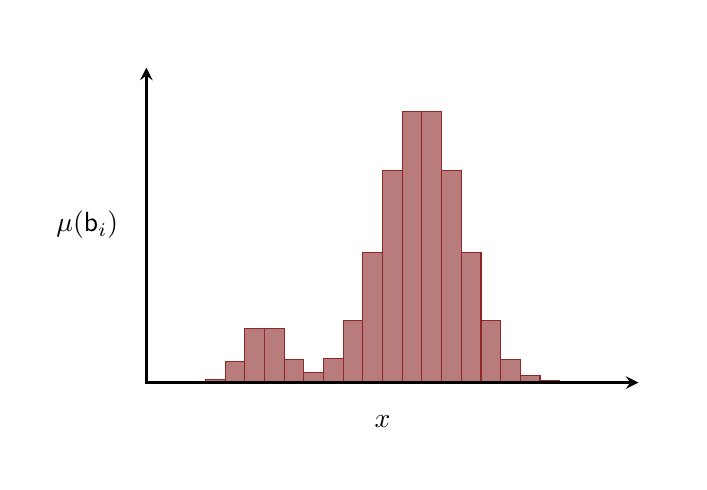
\begin{tikzpicture}[scale=1]
  \draw[white] (-4.5, -3) rectangle (3.75, 2.5);
  
  \foreach \l/\u/\m in {-3.000000/-2.750000/0.000000, -2.750000/-2.500000/0.000003, -2.500000/-2.250000/0.000132, -2.250000/-2.000000/0.002140, -2.000000/-1.750000/0.013593, -1.750000/-1.500000/0.034160, -1.500000/-1.250000/0.034315, -1.250000/-1.000000/0.014596, -1.000000/-0.750000/0.006514, -0.750000/-0.500000/0.015018, -0.500000/-0.250000/0.039655, -0.250000/0.000000/0.082663, 0.000000/0.250000/0.134894, 0.250000/0.500000/0.172316, 0.500000/0.750000/0.172316, 0.750000/1.000000/0.134894, 1.000000/1.250000/0.082663, 1.250000/1.500000/0.039651, 1.500000/1.750000/0.014886, 1.750000/2.000000/0.004374, 2.000000/2.250000/0.001006, 2.250000/2.500000/0.000181, 2.500000/2.750000/0.000025, 2.750000/3.000000/0.000003} {
    \filldraw[fill=mid, draw=dark] (\l, -2) rectangle (\u, {(20 * \m - 2)});
  }
  
  \draw[->, >=stealth, line width=1] (-3, -2.0175) -- (-3, +2);
  \draw[->, >=stealth, line width=1] (-3, -2) -- (+3.25, -2);
  \node at (0, -2.5) { $x$ };
  \node at (-3.75, 0) { $\mu(\mathsf{b}_{i})$ };
  
\end{tikzpicture}

\end{document}  